\documentclass[a4paper,UKenglish,cleveref, autoref, thm-restate]{lipics-v2021}
\hideLIPIcs

\newcommand{\ident}[1]{\textsf{#1}}
\newcommand{\ddident}[1]{\guillemotleft\ident{#1}\guillemotright}
\newcommand{\sigmaN}{\sigma_0}
\newcommand{\select}{\textnormal{\ident{choose}}}
\newcommand{\choices}{\textnormal{\ident{choices}}}
\newcommand{\op}{\textit{op}}
\newcommand{\vect}[1]{\lbrack #1 \rbrack}
%\newcommand{\preview}{\textnormal{\ident{preview}}}
%\newcommand{\links}{\textnormal{\ident{links}}}
%\newcommand{\argmax}{\textit{arg}\,\textit{max}\,}

\bibliographystyle{plainurl}
\title{The Choose-Your-Own-Adventure Calculus (Pearl/Brave New Idea)}

\author{Tomas Petricek}{Charles University, Prague, Czechia}{tomas@tomasp.net}{0000-0002-7242-2208}{}
\author{Jan Liam Verter}{Charles University, Prague, Czechia}{todo@todo}{}{}
\author{Mikoláš Fromm}{Charles University, Prague, Czechia}{todo@todo}{}{}
\ccsdesc[500]{Software and its engineering~General programming languages}
\keywords{Interactive programming systems, Type providers, Proof assistants}
\nolinenumbers

% \funding{funding}
% \acknowledgements{I want to thank \dots}
\authorrunning{Authors}

\begin{document}

\maketitle

\begin{abstract}

Some of the most remarkable results in mathematics reveal connections between different
branches of the discipline. The aim of this paper is to point out a modest, but still
remarkable, similarity between a range of different interactive programming systems.

~

use a simple formal mathematical model
that we call \emph{the choose-your-own-adventure calculus} to


todo

% and enable a transfer of ideas between them

\end{abstract}

\newpage

\section{Introduction}

Multiple interactive programming systems, ranging from code editors for object-oriented programming
languages to data exploration systems and interactive proof assistants, exhibit a remarkably
similar pattern of interaction. They offer the user, who can be a programmer, a data scientist
or a proof writer, a range of choices that the user can select from in order to complete their
program, script or proof. The user can initiate the interaction iteratively, using it to
create and refine a larger part of their program.

There are subtle differences between different implementations of the general pattern. In some
systems, the resulting source code will contain a trace of the choices made by the user.
For example, when choosing an item from a list of class members, the code will contain the member
name. In some systems, the interaction results in a block of code that can be included in the
source file, but does not include a trace of the interaction. For example, invoking a proof search
or case split in Idris \cite{brady-2015-idris} constructs a well-typed program, but leaves no trace
of the command used to construct it.
%
The nature of the generated options also varies. The list of choices may include all possible
options that are valid at a given location, or it may list only a subset of the valid options.
In some cases, it may also include incorrect options as, for example, in auto-completion
for dynamic languages \cite{frolich-2024-autocomplete}.

The aim of this paper is paper is to formally capture the recurring interaction pattern:

\begin{enumerate}
\setlength{\itemsep}{5pt}
\item We motivate the formalism by reviewing four different systems that implement a variation on the
interaction pattern. These include type providers for data access in F\# \cite{syme-2013-inforich},
type providers for data exploration in The Gamma \cite{petricek-2022-thegamma,petricek-2017-dotdriven},
AI assistants for semi-automated data wrangling \cite{petricek-2023-aias} and tooling for
interactive proof assistants \cite{altenkirch-1994-alf,brady-2015-idris,verter-2024-mixed} (Section~\ref{sec:motivation}).

\item We introduce the \emph{choose-your-own-adventure calculus}, which is a small formal structure
that models an interactive system where a user constructs a program by repeatedly choosing from a list
of options offered by the system (Section~\ref{sec:calculus}).

\item The calculus allows us to make the aforementioned subtle differences precise. We define the
notions of \emph{correctness} and \emph{completeness} for the choose-your-own-adventure calculus.
To distinguish the different ways of embedding the interactions in the edited programs, we
also formally define \emph{internal} and \emph{external} mode of system integration.

\item We show that various programmer assistance tools, such as search and AI-based recommendations
can be built on top of the primitives offered by the calculus, showing how the
choose-your-own-adventure calculus supports of transfer of ideas across different kinds of
interactive programming systems.
\end{enumerate}

The main contribution of this paper is conceptual rather than technical. We capture a
pattern that is perhaps not surprising in retrospect, but that is easy to overlook until it is
given a name. We use formal programming language theory methods to precisely describe
interesting aspects of the pattern. Moreover, our work also confirms that programming
language theory methods can be extremely effective for studying not just \emph{programming
languages}, but also interactive \emph{programming systems}~\cite{jakubovic-2023-techdims}.

\newpage

\begin{figure}[t]
  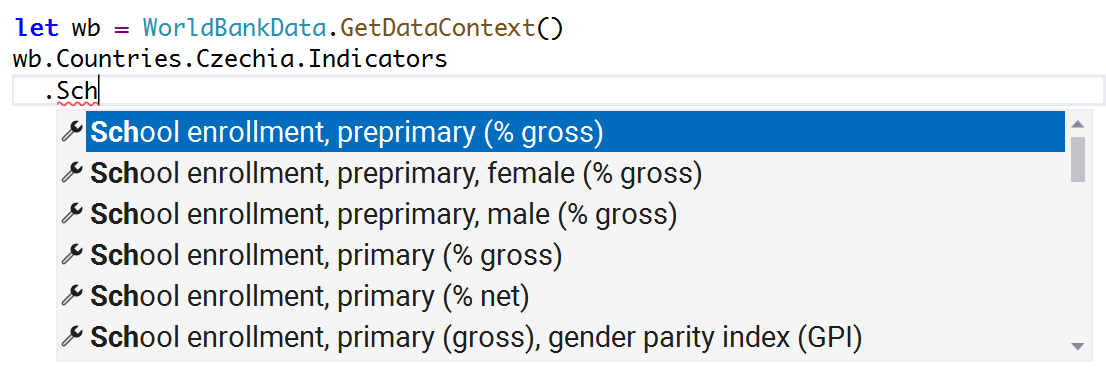
\includegraphics[width=0.7\textwidth]{fig/worldbank.png}
  \caption{F\# code editor showing completions offered by the World Bank type provider.}
  \label{fig:worldbank}
\end{figure}

\section{Motivation}
\label{sec:motivation}

Computer scientists studying programming have long focused on programming languages as syntactic
entities, sometimes neglecting the interactive environments in which they are inevitably
embedded \cite{rpg-2012-revolution}. Notably, in many of the motivating examples that we draw
from in this section, the interactive aspect of the system is only described in supplementary
materials \cite{brady-2015-idris,syme-2013-inforich,altenkirch-1994-alf}. Only recently, programming
language theory started to be used to study interactive environments
\cite{adams-2025-grove,mayer-2018-bidirectional}. Our work contributes to this research direction.

The following sections review four different instances of the choose-your-own-adventure
interaction pattern. In all of those, an interactive editor offers the user some kind of~a~com\-pletion list during working with the system.

\subparagraph{Type providers.}

F\# type providers \cite{syme-2013-inforich} are a mechanism for integrating external data
sources into the F\# type system. A type provider is a compiler extension, loaded and
executed at compile-time and at edit-time. It can run arbitrary code to read the structure of
external data and use it to generate a suitable statically-typed representation of the
data, typically as objects with members. Type providers can, for example, infer the type from a
sample JSON \cite{petricek-2016-fsdata} or read a database schema.

The example in Figure~\ref{fig:worldbank} shows a simple type provider for accessing information
from the World Development Indicators database. The provided \ident{wb} object allows the programmer
to access any indicator of any country in the database by choosing an appropriate \ident{[Country]}
and an \ident{[Indicator]} in a chain of members
\ident{wb}.\ident{Countries}.\ident{[Country]}.\ident{Indicator}.\ident{[Indicator]}.
The result is a time series with values for the given indicator and a country. More generally,
the example can be seen as a special case of a type provider for slicing n-dimensional
data cube \cite{petricek-2022-thegamma} -- we choose a fixed value for two of the three
dimensions (country, indicator, time).

When using the type provider, the user types the first line of code and triggers auto-completion
by typing \ident{wb} followed by the dot. The rest of the code is constructed by choosing an
option from a list and typing another dot.\footnote{This interaction pattern has been
lightheartedly called \emph{dot-driven development} by Phil Trelford \cite{seemann-2021-head}.}


\newpage

\begin{figure}[t]
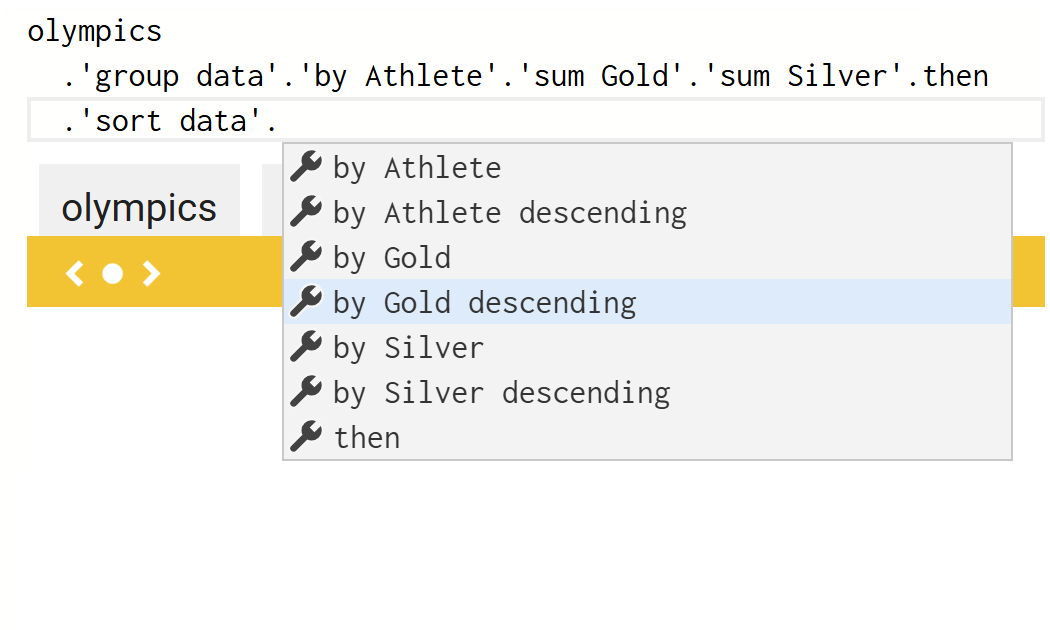
\includegraphics[width=0.48\textwidth]{fig/thegamma1.png}~~
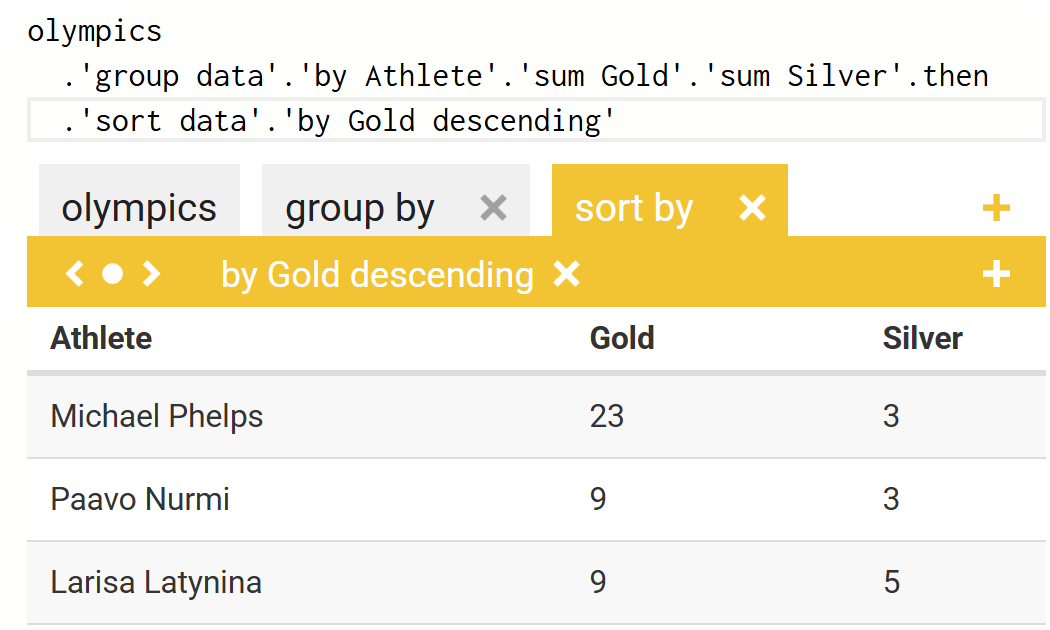
\includegraphics[width=0.48\textwidth]{fig/thegamma2.png}
\caption{Constructing a query in The Gamma. We count the number of gold and silver medals for
each athlete and sort the data by the number of gold medals.}
\label{fig:thegamma}
\end{figure}

\subparagraph{Data exploration.}

The Gamma~\cite{petricek-2022-thegamma} is a programmatic data exploration environment
for non-programmers. In The Gamma, type providers are the primary programming mechanism. They
are used not just for data access, but also for constructing queries.

The type provider shown in Figure~\ref{fig:thegamma} lets the user construct an SQL-like query by
repeatedly choosing operations and their parameters \cite{petricek-2017-dotdriven}. It keeps track
of the schema and uses it to generate all possible valid parameters. When sortin data, it generates
an object with two members for each columns -- one for ascending and one for descending sort.
Similarly, the grouping operation first offers all columns as possible grouping keys and then
lets the user choose from a range of pre-defined aggregations (sum, count, average, concatenate).
The system also evaluates the query on the fly, providing a live preview during editing \cite{petricek-2020-live}.

The interaction pattern is the same as before. After the usertriggers auto-completion, they
repeatedly select an operation and its parameters to construct a query. One notable difference
is that the structure of the generated types is potentially infinite (the user can keep adding
further operations) and so the types are generated lazily.

\subparagraph{AI assistants.}

The third instance of the choose-your-own-adventure interaction pattern comes from the work on
semi-automatic data wrangling tools known as AI assistants \cite{petricek-2023-aias}.
An AI assistant guides the analyst through a data wrangling problem such as reconciling mismatched
datasets, filling missing values or inferring data format and types. An AI assistant solves
the problem automatically and suggests an initial data transformation, but it also generates a
number of constraints that the user can choose from to refine the initial solution. If the initial
solution is not correct, the user chooses a constraint and the AI assistant runs again, suggesting
a new data transformation that respects the constraint.

Figure~\ref{fig:aia} shows an example. It uses the datadiff \cite{sutton-2018-datadiff} AI
assistant, running in a Wrattler notebook \cite{petricek-2018-wrattler}, to merge broadband
quality data published by Ofcom for two subsequent years. The format of the CSV files for the
two years differs. Columns were added, removed, renamed and their order has changed. In the
example, we selected 6 columns from the year 2015 and want to find matching data from 2014.

When the AI assistants runs automatically, it correctly maps the numerical columns, but it
incorrectly maps the \ident{Urban.rural} (2014) column to \ident{Nation} (2015). This happens
because both columns are categorical and have three values with similar distribution. A data
analyst can easily spot the mistake. They click the ``+'' button to add a constraint and choose
\ident{Don't match Urban.rural and Nation} to specify that the two columns should not be matched.
Datadiff then runs again and finds the correct matching.

\begin{figure}[t]
  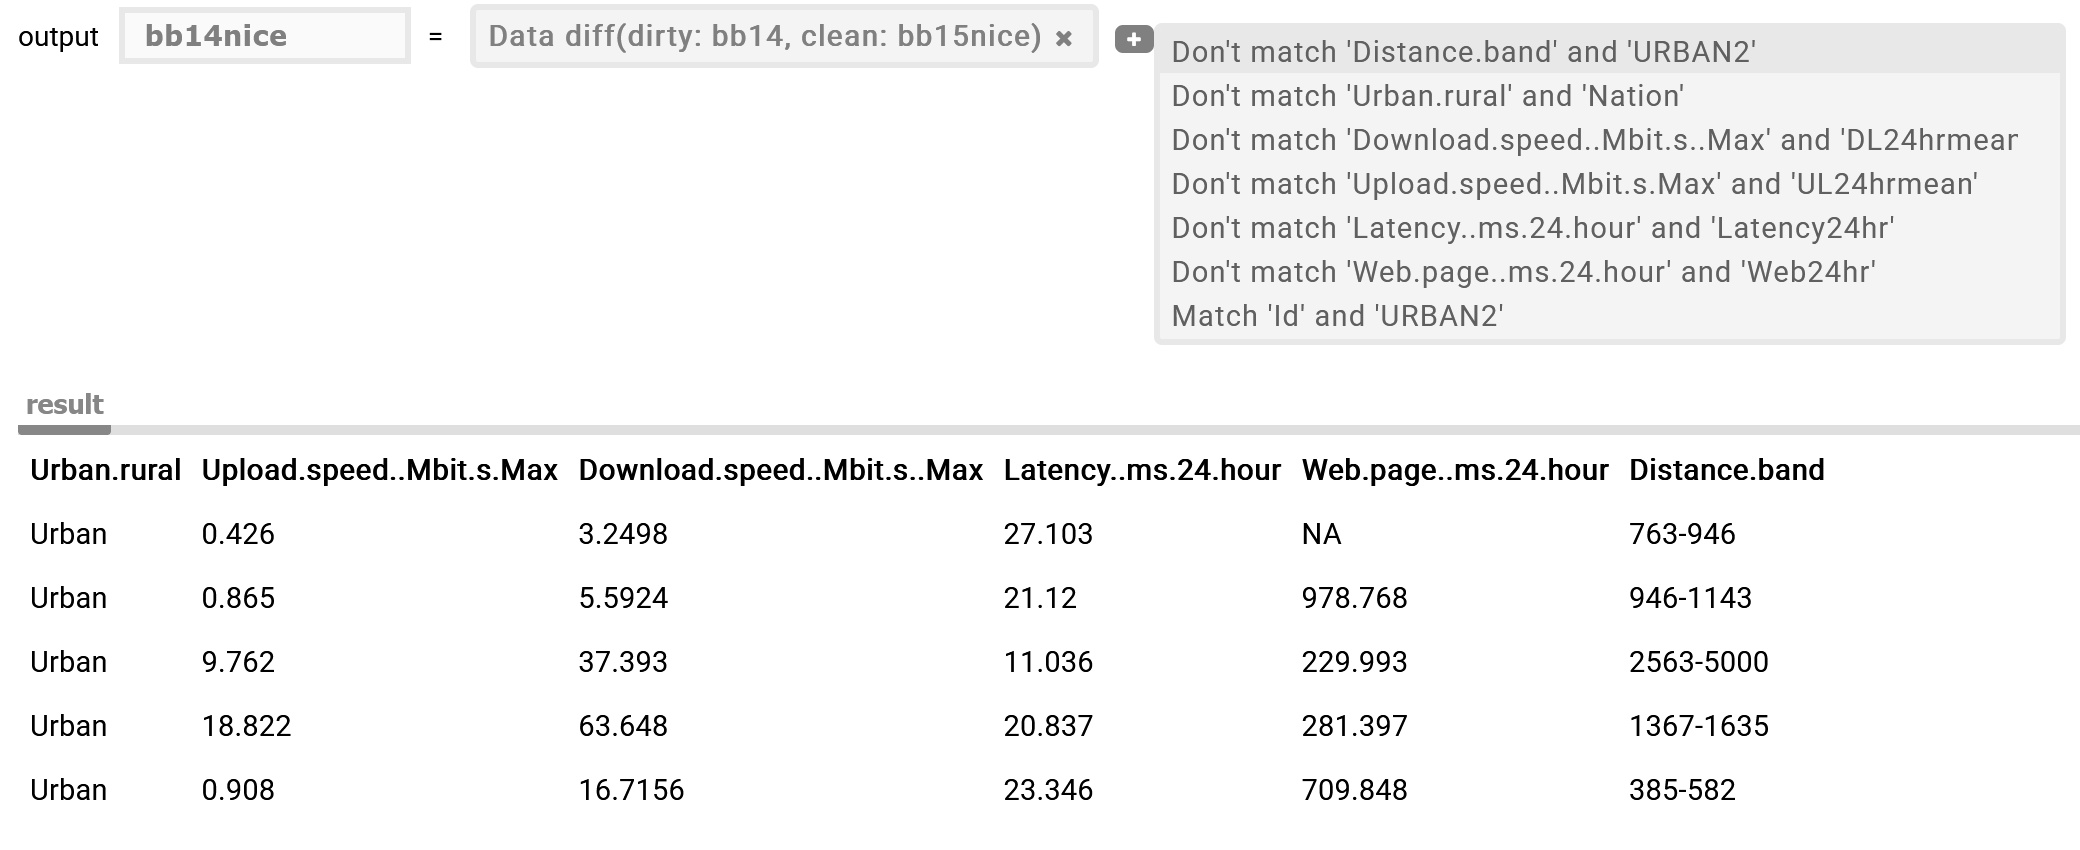
\includegraphics[width=0.9\textwidth]{fig/aia.png}
  \caption{Using the datadiff AI assistant to reconcile the structure of the two datasets.
    The user is offered a list of constraints to prevent or force matching between specific columns.}
  \label{fig:aia}
\end{figure}

~

The interaction patter is the same as in the previous two cases. The analyst constructs the
correct data transformation by repeatedly choosing from a list of options, until they obtain
the desired result. However, the way the interaction pattern is implemented differs.
First, in the case of type providers, we are gradually constructing a program by adding operations to
a method chain. Now, the AI assistant synthesizes a data transformation (program) and we are
gradually adding constraints to control the synthesis. Second, in the case of type providers,
the completion list offered all possible members of the object. Now, the list offers
constraints recommended by the AI assistant which may not be complete.

\newpage

\begin{figure}[t]
  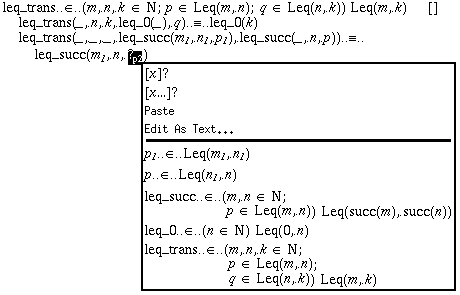
\includegraphics[width=0.6\textwidth]{fig/alf.png}
  \caption{Constructing a proof of the transitivity of the $\leq$ relation in the \textsc{Alf}
    editor. The user is offered a range of variables and constructors in scope at the current
    location. \cite{altenkirch-1994-alf}}
  \label{fig:alf}
\end{figure}


\subparagraph{Interactive theorem provers.}
A fourth example of the choose-your-own-adventure interactive pattern can be found in interactive
theorem provers. When writing programs in systems like Idris \cite{brady-2021-idris2}, the
user typically works by stating the desired conclusion and filling the implementation with a hole.
The system provides a range of interactive editing capabilities to fill the holes \cite{mcbride-1999-dependently}.
It can, for example, generate a case split or search for a proof \cite{brady-2015-idris}.

Systems like Idris provide key bindings to invoke the completions, but the functionality could
also be offered through a user interface. An example that illustrates this is the interactive editor
for the \textsc{Alf} theorem prover \cite{magnusson-1994-alf}, which is based on the refinement of
an incomplete proof object \cite{altenkirch-1994-alf}. This is illustrated in Figure~\ref{fig:alf}.
The user is proving the transitivity of the $\leq$ relation for Peano arithmetic natural numbers.
They pattern match on the proof argument $p$ and complete the first branch. For the second branch,
they need to fill a hole $?_{p2}$ (called a wildcard in \textsc{Alf}). They trigger a completion
and a pop-up menu shows the available variables and constructors, including \ident{leq\_trans} that
can be used to complete the proof. After choosing \ident{leq\_trans}, two new holes are generated
for its arguments. Those can be, again, filled interactively, by choosing $p_1$ and $p$ from the
completion.

The interaction pattern is again the same. The user repeatedly triggers a completion and uses
it to refine and complete their proof by filling holes. There are subtle differences too. Unlike
with AI assistants, each completion directly refines the proof that the user is editing. Unlike
with type providers, a completion may generate multiple new holes, rather than just adding to a
chain of operations.

The \textsc{Alf} editor is a historical example, but a similar user interface could be built for
systems like Idris or Coq. The two would work differently. As in \textsc{Alf}, Idris source code
represents the proof itself and a completion would replace a hole with a suggested term. In Coq,
the proof is a series of tactic invocations and so selected completions would be added to this
list and would form a trace of the interaction with the user.

\newpage

\section{Formal model}
\label{sec:calculus}

A system that implements the choose-your-own-adventure interaction pattern repeatedly offers
the user a range of options to choose from. Each of the options is designated by an identifier.
The system also maintains a state during the process which determines subsequent options. The state
may not be visible to the user, but the user can always explicitly request the program constructed
so far.

We can think of the interaction with the system as navigating through a tree structure, starting
from a root and choosing one of the possible branches in each step.\footnote{Serving as another
evidence for the surprising effectiveness of the concept of a tree \cite{nesetril-2005-strom}.}
In the following definition, the key $\choices$ operation can thus be seen as returning
branches of a given node.

\begin{definition}[Choose-your-own-adventure system]\label{def:calculus}
Given expressions $e\in \mathbb{E}$ and states $\sigma \in \Sigma$, a choose-your-own-adventure
system is a pair of operations \choices, \select\ such that:

\vspace{-0.25em}
\begin{itemize}
  \item $\choices(\sigma) = (\iota_1\mapsto\sigma_1, \ldots, \iota_n\mapsto\sigma_n)$ is
    an operation that takes a state and generates options designated by an identifier $\iota_i$
    and represented by a state $\sigma_i$,
  \item $\select(\sigma) = e$ is an operation that returns generated program for a given state.
\end{itemize}
\end{definition}

The definition is not a programming language calculus in the usual sense in that it does not
define a concrete syntax with reduction rules. It is an abstract algebraic structure that captures
the structure of a system that supports the choose-your-own-adventure interaction pattern.
The definition is close to that of an AI assistant \cite{petricek-2023-aias}, which is written
using a language specific for the data wrangling domain (such as cleaning scripts or input and
output data) but is structurally similar. It is also worth noting that the definition may describe
not just trees, but also graphs with cycles -- a system can return to an already visited state.
This is not practically useful, but it does not pose a theoretical problem.

\subparagraph{External mode of embedding.}
One of the subtle questions about the choose-your-own-adventure pattern raised in the introduction
concerns the different ways in which a trace of the interaction is embedded in the interactively
constructed program. In the \emph{external mode}, the interaction results in code that becomes a
part of the edited program, but it is not possible to reconstruct the steps used to generate the code.

The choose-your-own-adventure interaction pattern is typically used to complete a partial program.
To model this, we assume that the host language has a notion of a hole, written as~$?$
and that a user can select a part of program to invoke the completion on. We write $E[e]$ for a
completion context, akin to evaluation contexts in operational semantics.

We assume that, for a program containing a hole in a completion context $E[?]$, we can construct
an initial choose-your-own-adventure state using an operation
$\ident{init}(E[?])=\sigmaN$.

\begin{definition}\label{def:external}
An expression $E[?]$ is completed as $E[e]$ via external embedding of an interaction with
a choose-your-own-adventure system consisting of \choices\ and \select\ if:

\vspace{-0.25em}
\raggedright
\begin{enumerate}
\item $\ident{init}(E[?]) = \sigmaN$ obtains the initial state of a choose-your-own-interaction system,
\item $\sigma_n$ is a system state such that $\forall i\in{1\ldots n}.(\iota_i\mapsto\sigma_i)\in\choices{(\sigma_{n-1})}$,
  i.e.,~the user\\ makes a series of choices resulting in a final state of the system $\sigma_n$,
\item $E[e]$ where $e=\select(\sigma_n)$, i.e.,~the final program is constructed by replacing the hole
  in the completion context with the expression $e$ generated from $\sigma_n$.
\end{enumerate}
\end{definition}

As we will see when we revisit the earlier examples formally, the external mode of embedding is
used, for example, in the case of interactive theorem provers like \textsc{Alf} or Idris.
In those systems, the user triggers the completion on a proof (program) containing a hole.
They then fill the hole and, possibly iteratively, further holes in the generated proof. The final
expression is embedded in the source code, but it does not indicate what options, identified by
$\iota_1, \ldots, \iota_n$, were selected in the process.

\subparagraph{Internal mode of embedding.}
In the \emph{internal mode}, a trace of the interaction with a choose-your-own-adventure system
is embedded directly in the constructed program. This is the case with type providers, where a
user chooses a sequence of object members to be accessed. The same would be the case in a completion
system for Coq that would offer tactics to apply, becuase the resulting proof would contain a
record of the selected tactics.

To talk about the internal mode formally, we again need the \ident{init} operation, but also an
operation \ident{decode} that extracts identifiers of invoked completions from an expression.
An internal embedding is the same as external embedding with an additional constraint:

\begin{definition}\label{def:internal}
An expression $E[?]$ is completed as $E[e]$ via internal embedding of an interaction with
a choose-your-own-adventure system consisting of \choices\ and \select\ if:

\vspace{-0.25em}
\raggedright
\begin{enumerate}
\item $E[?]$ is completed as $E[e]$ via external embedding using \ident{init}, \choices\ and \select\\
  through a series of choices designated by identifiers $\iota_1, \ldots, \iota_n$,
\item it also holds that $\ident{decode}(e)=(\iota_1, \ldots, \iota_n)$.
\end{enumerate}
\end{definition}

If a choose-your-own-adventure system is integrated in a programming language
through internal embedding, we can reconstruct the choices through which the user constructed
an expression $e$ in a completion context $E[e]$, assuming they used the interactive system rather
than entering the code directly. This also means that we can reconstruct the final state $\sigma_n$
of the system by starting from $\ident{init}(E[?])$ and following the choices specified by
$\iota_1, \ldots, \iota_n$.


\newpage
\section{Examples}
\label{sec:examples}

We now revisit the four examples from Section~\ref{sec:motivation} and show how they fit the
above formal model. All four examples rely on some domain-specific logic. We describe what
information the logic provides, but do not model it formally. This has been done elsewhere,
in works describing the individual systems.

To show how the model lets us distinguish subtle details of interactive programming systems,
we start with a model of data exploration system that is inspired by The Gamma, but differs in
one notable way. We then discuss type providers more generally and show how to correctly model
The Gamma. We then revisit the remaining two examples.

\subsection{Data exploration}

In The Gamma, the choose-your-own-adventure interaction pattern is used to construct a
query that transforms the given input data. The query is a sequence of operations with parameters,
$\op(p_1, \ldots, p_n)$, loosely modelled after relational algebra \cite{codd-1970-relational}.

In The Gamma, the query is hidden from the data analyst. Behind the scenes, the system generates
objects with members and the identifiers designating individual options are the names of those
members. The operation is encapsulated in the code of the accessor of the member. In the
simplified model in this section we ignore this fact. The model presented here directly
generates code that calls the underlying operations. For example, assume that the user makes
the following choices:
\[
\textnormal{\ddident{group data}\,.\,\ddident{by Athlete}\,.\,\ddident{sum Gold}\,.\,\ddident{count all}\,.\,\ddident{then}}
\]
In The Gamma, the individual identifiers become object members and they are included as
a member chain in the generated code. In the following simplified model, the completion
instead fills the hole with an expression representing the operation:
\[
\ident{group}(\texttt{"Athlete"}, \ident{sum}(\texttt{"Gold"}), \ident{count}())
\]
The two approaches have different human-computer interaction trade-offs. In terms of cognitive
dimensions \cite{green-1989-cogdims,blackwell-2003-cogdims}, the latter has a greater closeness
of mapping, while the former is less cognitively demanding to read for a non-programmer.
As discussed in Section~\ref{sec:properties}, the two implementations of the choose-your-own-adventure
interaction pattern also differ in terms of their formal properties.

\subparagraph{Formal model.}
The options generated by The Gamma let the user select both the next operation and the parameters
of the previously selected operation. The available operations and parameters are generated
based on a schema $S$ that is transformed by the operations. The state of the system $\sigma$
contains the current schema $S$ and the operations applied so far. In the following, we write
$\op(\boldsymbol{p})$ for an operation with a vector of parameters:
\[
\sigma = S, \vect{\op_1(\boldsymbol{p_1}), \ldots, \op_n(\boldsymbol{p_n})}\\
\]
The behaviour of the $\choices$ operation depends on whether the last operation in the sequence
expects further parameters or whether it is fully-specified. In the first case, the recommendation
engine generates possible additional parameter values $p_', p_'', \ldots$ based on the schema $S$,
the operation $\op_n$ and the already known parameters $\boldsymbol{p_n}$.
The $\choices$ operation then generates options that add the additional parameter. We generated the
identifiers $\iota_',\iota_'',\ldots$ based on the state and the parameter value, such as
\ddident{by Gold descending}. Note that adding a parameter may also result in a new schema
$S', S'', \ldots$ (which the recommendation engine computes based on the previous schema and the new parameter):
\[
\begin{array}{l}
\choices(S, \vect{\op_1(\boldsymbol{p_1}), \ldots, \op_n(\boldsymbol{p_n})}) =\\
\qquad (S', \vect{\op_1(\boldsymbol{p_1}), \ldots, \op_n(\boldsymbol{p_n},p')}), \\
\qquad (S'', \vect{\op_1(\boldsymbol{p_1}), \ldots, \op_n(\boldsymbol{p_n},p'')}), ~\ldots
\end{array}
\]
If the last operation takes no further parameters, the system produces a choice
of possible next operations $\op', \op'', \ldots$. Again, we are also given new schemas $S', S'', \ldots$
and we generate identifiers $\iota',\iota'',\ldots$ based on the operation name. The $\ident{choices}$
operation then returns options that add the additional operation:
\[
\begin{array}{l}
\choices(S, (\op_1(\boldsymbol{p_1}), \ldots, \op_n(\boldsymbol{p_n}))) =\\
\qquad (S', \vect{\op_1(\boldsymbol{p_1}), \ldots, \op_n(\boldsymbol{p_n}), \op'()}), \\
\qquad (S'', \vect{\op_1(\boldsymbol{p_1}), \ldots, \op_n(\boldsymbol{p_n}), \op''()}), ~\ldots
\end{array}
\]
Finally, the $\select$ operation takes the state $\sigma$ and generates an expression that represents
the data transformation. This is only possible if all parameters are fully-specified. For simplicity,
assume that $k$ is the index of the last fully-specified operation (either $n$ or $n-1$). If the
host language lets us compose functions using $f\circ g$, we can write:
\[
\select(S, (\op_1(\boldsymbol{p_1}), \ldots, \op_n(\boldsymbol{p_n}))) = \op_1(\boldsymbol{p_1}) \circ \ldots \circ \op_k(\boldsymbol{p_k})
\]
The recommendation engine behind The Gamma provides a domain-specific logic for generating
possible operations and their parameters based on the current schema of the data. As the above
definition shows, this underlying engine can be easily exposed through the common
choose-your-own-adventure interface.

\subsection{Type providers}

revisit

~

\subsection{AI assistants}

~

\subsection{Interactive theorem proving}
~

The internal mode can also be used when
working with theorem provers.

In Coq, where proofs are represented as series of tactics,

However, this would also be case in a
completion engine for the Coq proof system that would offer a choice of tactics to apply, because
Coq proofs are represented

~

\newpage

\section{Properties}
\label{sec:properties}

~

\section{Applications}
\label{sec:applications}


\cite{rein-2019-exploratory}

\newpage

\bibliography{paper}

\newpage

\section{Typesetting instructions -- Summary}
\label{sec:typesetting-summary}

LIPIcs is a series of open access high-quality conference proceedings across all fields in informatics established in cooperation with Schloss Dagstuhl.
In order to do justice to the high scientific quality of the conferences that publish their proceedings in the LIPIcs series, which is ensured by the thorough review process of the respective events, we believe that LIPIcs proceedings must have an attractive and consistent layout matching the standard of the series.
Moreover, the quality of the metadata, the typesetting and the layout must also meet the requirements of other external parties such as indexing service, DOI registry, funding agencies, among others. The guidelines contained in this document serve as the baseline for the authors, editors, and the publisher to create documents that meet as many different requirements as possible.

Please comply with the following instructions when preparing your article for a LIPIcs proceedings volume.
\paragraph*{Minimum requirements}

\begin{itemize}
\item Use pdflatex and an up-to-date \LaTeX{} system.
\item Use further \LaTeX{} packages and custom made macros carefully and only if required.
\item Use the provided sectioning macros: \verb+\section+, \verb+\subsection+, \verb+\subsubsection+, \linebreak \verb+\paragraph+, \verb+\paragraph*+, and \verb+\subparagraph*+.
\item Provide suitable graphics of at least 300dpi (preferably in PDF format).
\item Use BibTeX and keep the standard style (\verb+plainurl+) for the bibliography.
\item Please try to keep the warnings log as small as possible. Avoid overfull \verb+\hboxes+ and any kind of warnings/errors with the referenced BibTeX entries.
\item Use a spellchecker to correct typos.
\end{itemize}

\paragraph*{Mandatory metadata macros}
Please set the values of the metadata macros carefully since the information parsed from these macros will be passed to publication servers, catalogues and search engines.
Avoid placing macros inside the metadata macros. The following metadata macros/environments are mandatory:
\begin{itemize}
\item \verb+\title+ and, in case of long titles, \verb+\titlerunning+.
\item \verb+\author+, one for each author, even if two or more authors have the same affiliation.
\item \verb+\authorrunning+ and \verb+\Copyright+ (concatenated author names)\\
The \verb+\author+ macros and the \verb+\Copyright+ macro should contain full author names (especially with regard to the first name), while \verb+\authorrunning+ should contain abbreviated first names.
\item \verb+\ccsdesc+ (ACM classification, see \url{https://www.acm.org/publications/class-2012}).
\item \verb+\keywords+ (a comma-separated list of keywords).
\item \verb+\relatedversion+ (if there is a related version, typically the ``full version''); please make sure to provide a persistent URL, e.\,g., at arXiv.
\item \verb+\begin{abstract}...\end{abstract}+ .
\end{itemize}

\paragraph*{Please do not \ldots} %Do not override the \texttt{\seriesstyle}-defaults}
Generally speaking, please do not override the \texttt{lipics-v2021}-style defaults. To be more specific, a short checklist also used by Dagstuhl Publishing during the final typesetting is given below.
In case of \textbf{non-compliance} with these rules Dagstuhl Publishing will remove the corresponding parts of \LaTeX{} code and \textbf{replace it with the \texttt{lipics-v2021} defaults}. In serious cases, we may reject the LaTeX-source and expect the corresponding author to revise the relevant parts.
\begin{itemize}
\item Do not use a different main font. (For example, the \texttt{times} package is forbidden.)
\item Do not alter the spacing of the \texttt{lipics-v2021.cls} style file.
\item Do not use \verb+enumitem+ and \verb+paralist+. (The \texttt{enumerate} package is preloaded, so you can use
 \verb+\begin{enumerate}[(a)]+ or the like.)
\item Do not use ``self-made'' sectioning commands (e.\,g., \verb+\noindent{\bf My+ \verb+Paragraph}+).
\item Do not hide large text blocks using comments or \verb+\iffalse+ $\ldots$ \verb+\fi+ constructions.
\item Do not use conditional structures to include/exclude content. Instead, please provide only the content that should be published -- in one file -- and nothing else.
\item Do not wrap figures and tables with text. In particular, the package \texttt{wrapfig} is not supported.
\item Do not change the bibliography style. In particular, do not use author-year citations. (The
\texttt{natbib} package is not supported.)
\end{itemize}

\enlargethispage{\baselineskip}

This is only a summary containing the most relevant details. Please read the complete document ``LIPIcs: Instructions for Authors and the \texttt{lipics-v2021} Class'' for all details and don't hesitate to contact Dagstuhl Publishing (\url{mailto:publishing@dagstuhl.de}) in case of questions or comments:
\href{http://drops.dagstuhl.de/styles/lipics-v2021/lipics-v2021-authors/lipics-v2021-authors-guidelines.pdf}{\texttt{http://drops.dagstuhl.de/styles/lipics-v2021/\newline lipics-v2021-authors/lipics-v2021-authors-guidelines.pdf}}

\section{Lorem ipsum dolor sit amet}

Lorem ipsum dolor sit amet, consectetur adipiscing elit \cite{DBLP:journals/cacm/Knuth74}. Praesent convallis orci arcu, eu mollis dolor. Aliquam eleifend suscipit lacinia. Maecenas quam mi, porta ut lacinia sed, convallis ac dui. Lorem ipsum dolor sit amet, consectetur adipiscing elit. Suspendisse potenti. Donec eget odio et magna ullamcorper vehicula ut vitae libero. Maecenas lectus nulla, auctor nec varius ac, ultricies et turpis. Pellentesque id ante erat. In hac habitasse platea dictumst. Curabitur a scelerisque odio. Pellentesque elit risus, posuere quis elementum at, pellentesque ut diam. Quisque aliquam libero id mi imperdiet quis convallis turpis eleifend.

\begin{lemma}[Lorem ipsum]
\label{lemma:lorem}
Vestibulum sodales dolor et dui cursus iaculis. Nullam ullamcorper purus vel turpis lobortis eu tempus lorem semper. Proin facilisis gravida rutrum. Etiam sed sollicitudin lorem. Proin pellentesque risus at elit hendrerit pharetra. Integer at turpis varius libero rhoncus fermentum vitae vitae metus.
\end{lemma}

\begin{proof}
Cras purus lorem, pulvinar et fermentum sagittis, suscipit quis magna.


\proofsubparagraph*{Just some paragraph within the proof.}
Nam liber tempor cum soluta nobis eleifend option congue nihil imperdiet doming id quod mazim placerat facer possim assum. Lorem ipsum dolor sit amet, consectetuer adipiscing elit, sed diam nonummy nibh euismod tincidunt ut laoreet dolore magna aliquam erat volutpat.
\begin{claim}
content...
\end{claim}
\begin{claimproof}
content...
    \begin{enumerate}
        \item abc abc abc \claimqedhere{}
    \end{enumerate}
\end{claimproof}

\end{proof}

\begin{corollary}[Curabitur pulvinar, \cite{DBLP:books/mk/GrayR93}]
\label{lemma:curabitur}
Nam liber tempor cum soluta nobis eleifend option congue nihil imperdiet doming id quod mazim placerat facer possim assum. Lorem ipsum dolor sit amet, consectetuer adipiscing elit, sed diam nonummy nibh euismod tincidunt ut laoreet dolore magna aliquam erat volutpat.
\end{corollary}

\begin{proposition}\label{prop1}
This is a proposition
\end{proposition}

\autoref{prop1} and \cref{prop1} \ldots

\subsection{Curabitur dictum felis id sapien}

Curabitur dictum \cref{lemma:curabitur} felis id sapien \autoref{lemma:curabitur} mollis ut venenatis tortor feugiat. Curabitur sed velit diam. Integer aliquam, nunc ac egestas lacinia, nibh est vehicula nibh, ac auctor velit tellus non arcu. Vestibulum lacinia ipsum vitae nisi ultrices eget gravida turpis laoreet. Duis rutrum dapibus ornare. Nulla vehicula vulputate iaculis. Proin a consequat neque. Donec ut rutrum urna. Morbi scelerisque turpis sed elit sagittis eu scelerisque quam condimentum. Pellentesque habitant morbi tristique senectus et netus et malesuada fames ac turpis egestas. Aenean nec faucibus leo. Cras ut nisl odio, non tincidunt lorem. Integer purus ligula, venenatis et convallis lacinia, scelerisque at erat. Fusce risus libero, convallis at fermentum in, dignissim sed sem. Ut dapibus orci vitae nisl viverra nec adipiscing tortor condimentum \cite{DBLP:journals/cacm/Dijkstra68a}. Donec non suscipit lorem. Nam sit amet enim vitae nisl accumsan pretium.

\begin{lstlisting}[caption={Useless code.},label=list:8-6,captionpos=t,float,abovecaptionskip=-\medskipamount]
for i:=maxint to 0 do
begin
    j:=square(root(i));
end;
\end{lstlisting}

\subsection{Proin ac fermentum augue}

Proin ac fermentum augue. Nullam bibendum enim sollicitudin tellus egestas lacinia euismod orci mollis. Nulla facilisi. Vivamus volutpat venenatis sapien, vitae feugiat arcu fringilla ac. Mauris sapien tortor, sagittis eget auctor at, vulputate pharetra magna. Sed congue, dui nec vulputate convallis, sem nunc adipiscing dui, vel venenatis mauris sem in dui. Praesent a pretium quam. Mauris non mauris sit amet eros rutrum aliquam id ut sapien. Nulla aliquet fringilla sagittis. Pellentesque eu metus posuere nunc tincidunt dignissim in tempor dolor. Nulla cursus aliquet enim. Cras sapien risus, accumsan eu cursus ut, commodo vel velit. Praesent aliquet consectetur ligula, vitae iaculis ligula interdum vel. Integer faucibus faucibus felis.

\begin{itemize}
\item Ut vitae diam augue.
\item Integer lacus ante, pellentesque sed sollicitudin et, pulvinar adipiscing sem.
\item Maecenas facilisis, leo quis tincidunt egestas, magna ipsum condimentum orci, vitae facilisis nibh turpis et elit.
\end{itemize}

\begin{remark}
content...
\end{remark}

\section{Pellentesque quis tortor}

Nec urna malesuada sollicitudin. Nulla facilisi. Vivamus aliquam tempus ligula eget ornare. Praesent eget magna ut turpis mattis cursus. Aliquam vel condimentum orci. Nunc congue, libero in gravida convallis \cite{DBLP:conf/focs/HopcroftPV75}, orci nibh sodales quam, id egestas felis mi nec nisi. Suspendisse tincidunt, est ac vestibulum posuere, justo odio bibendum urna, rutrum bibendum dolor sem nec tellus.

\begin{lemma} [Quisque blandit tempus nunc]
Sed interdum nisl pretium non. Mauris sodales consequat risus vel consectetur. Aliquam erat volutpat. Nunc sed sapien ligula. Proin faucibus sapien luctus nisl feugiat convallis faucibus elit cursus. Nunc vestibulum nunc ac massa pretium pharetra. Nulla facilisis turpis id augue venenatis blandit. Cum sociis natoque penatibus et magnis dis parturient montes, nascetur ridiculus mus.
\end{lemma}

Fusce eu leo nisi. Cras eget orci neque, eleifend dapibus felis. Duis et leo dui. Nam vulputate, velit et laoreet porttitor, quam arcu facilisis dui, sed malesuada risus massa sit amet neque.

\section{Morbi eros magna}

Morbi eros magna, vestibulum non posuere non, porta eu quam. Maecenas vitae orci risus, eget imperdiet mauris. Donec massa mauris, pellentesque vel lobortis eu, molestie ac turpis. Sed condimentum convallis dolor, a dignissim est ultrices eu. Donec consectetur volutpat eros, et ornare dui ultricies id. Vivamus eu augue eget dolor euismod ultrices et sit amet nisi. Vivamus malesuada leo ac leo ullamcorper tempor. Donec justo mi, tempor vitae aliquet non, faucibus eu lacus. Donec dictum gravida neque, non porta turpis imperdiet eget. Curabitur quis euismod ligula.


%%
%% Bibliography
%%

%% Please use bibtex,

\bibliography{lipics-v2021-sample-article}

\appendix

\section{Styles of lists, enumerations, and descriptions}\label{sec:itemStyles}

List of different predefined enumeration styles:

\begin{itemize}
\item \verb|\begin{itemize}...\end{itemize}|
\item \dots
\item \dots
%\item \dots
\end{itemize}

\begin{enumerate}
\item \verb|\begin{enumerate}...\end{enumerate}|
\item \dots
\item \dots
%\item \dots
\end{enumerate}

\begin{alphaenumerate}
\item \verb|\begin{alphaenumerate}...\end{alphaenumerate}|
\item \dots
\item \dots
%\item \dots
\end{alphaenumerate}

\begin{romanenumerate}
\item \verb|\begin{romanenumerate}...\end{romanenumerate}|
\item \dots
\item \dots
%\item \dots
\end{romanenumerate}

\begin{bracketenumerate}
\item \verb|\begin{bracketenumerate}...\end{bracketenumerate}|
\item \dots
\item \dots
%\item \dots
\end{bracketenumerate}

\begin{description}
\item[Description 1] \verb|\begin{description} \item[Description 1]  ...\end{description}|
\item[Description 2] Fusce eu leo nisi. Cras eget orci neque, eleifend dapibus felis. Duis et leo dui. Nam vulputate, velit et laoreet porttitor, quam arcu facilisis dui, sed malesuada risus massa sit amet neque.
\item[Description 3]  \dots
%\item \dots
\end{description}

\cref{testenv-proposition} and \autoref{testenv-proposition} ...

\section{Theorem-like environments}\label{sec:theorem-environments}

List of different predefined enumeration styles:

\begin{theorem}\label{testenv-theorem}
Fusce eu leo nisi. Cras eget orci neque, eleifend dapibus felis. Duis et leo dui. Nam vulputate, velit et laoreet porttitor, quam arcu facilisis dui, sed malesuada risus massa sit amet neque.
\end{theorem}

\begin{lemma}\label{testenv-lemma}
Fusce eu leo nisi. Cras eget orci neque, eleifend dapibus felis. Duis et leo dui. Nam vulputate, velit et laoreet porttitor, quam arcu facilisis dui, sed malesuada risus massa sit amet neque.
\end{lemma}

\begin{corollary}\label{testenv-corollary}
Fusce eu leo nisi. Cras eget orci neque, eleifend dapibus felis. Duis et leo dui. Nam vulputate, velit et laoreet porttitor, quam arcu facilisis dui, sed malesuada risus massa sit amet neque.
\end{corollary}

\begin{proposition}\label{testenv-proposition}
Fusce eu leo nisi. Cras eget orci neque, eleifend dapibus felis. Duis et leo dui. Nam vulputate, velit et laoreet porttitor, quam arcu facilisis dui, sed malesuada risus massa sit amet neque.
\end{proposition}

\begin{conjecture}\label{testenv-conjecture}
Fusce eu leo nisi. Cras eget orci neque, eleifend dapibus felis. Duis et leo dui. Nam vulputate, velit et laoreet porttitor, quam arcu facilisis dui, sed malesuada risus massa sit amet neque.
\end{conjecture}

\begin{observation}\label{testenv-observation}
Fusce eu leo nisi. Cras eget orci neque, eleifend dapibus felis. Duis et leo dui. Nam vulputate, velit et laoreet porttitor, quam arcu facilisis dui, sed malesuada risus massa sit amet neque.
\end{observation}

\begin{exercise}\label{testenv-exercise}
Fusce eu leo nisi. Cras eget orci neque, eleifend dapibus felis. Duis et leo dui. Nam vulputate, velit et laoreet porttitor, quam arcu facilisis dui, sed malesuada risus massa sit amet neque.
\end{exercise}

\begin{definition}\label{testenv-definition}
Fusce eu leo nisi. Cras eget orci neque, eleifend dapibus felis. Duis et leo dui. Nam vulputate, velit et laoreet porttitor, quam arcu facilisis dui, sed malesuada risus massa sit amet neque.
\end{definition}

\begin{example}\label{testenv-example}
Fusce eu leo nisi. Cras eget orci neque, eleifend dapibus felis. Duis et leo dui. Nam vulputate, velit et laoreet porttitor, quam arcu facilisis dui, sed malesuada risus massa sit amet neque.
\end{example}

\begin{note}\label{testenv-note}
Fusce eu leo nisi. Cras eget orci neque, eleifend dapibus felis. Duis et leo dui. Nam vulputate, velit et laoreet porttitor, quam arcu facilisis dui, sed malesuada risus massa sit amet neque.
\end{note}

\begin{note*}
Fusce eu leo nisi. Cras eget orci neque, eleifend dapibus felis. Duis et leo dui. Nam vulputate, velit et laoreet porttitor, quam arcu facilisis dui, sed malesuada risus massa sit amet neque.
\end{note*}

\begin{remark}\label{testenv-remark}
Fusce eu leo nisi. Cras eget orci neque, eleifend dapibus felis. Duis et leo dui. Nam vulputate, velit et laoreet porttitor, quam arcu facilisis dui, sed malesuada risus massa sit amet neque.
\end{remark}

\begin{remark*}
Fusce eu leo nisi. Cras eget orci neque, eleifend dapibus felis. Duis et leo dui. Nam vulputate, velit et laoreet porttitor, quam arcu facilisis dui, sed malesuada risus massa sit amet neque.
\end{remark*}

\begin{claim}\label{testenv-claim}
Fusce eu leo nisi. Cras eget orci neque, eleifend dapibus felis. Duis et leo dui. Nam vulputate, velit et laoreet porttitor, quam arcu facilisis dui, sed malesuada risus massa sit amet neque.
\end{claim}

\begin{claim*}\label{testenv-claim2}
Fusce eu leo nisi. Cras eget orci neque, eleifend dapibus felis. Duis et leo dui. Nam vulputate, velit et laoreet porttitor, quam arcu facilisis dui, sed malesuada risus massa sit amet neque.
\end{claim*}

\begin{proof}
Fusce eu leo nisi. Cras eget orci neque, eleifend dapibus felis. Duis et leo dui. Nam vulputate, velit et laoreet porttitor, quam arcu facilisis dui, sed malesuada risus massa sit amet neque.
\end{proof}

\begin{claimproof}
Fusce eu leo nisi. Cras eget orci neque, eleifend dapibus felis. Duis et leo dui. Nam vulputate, velit et laoreet porttitor, quam arcu facilisis dui, sed malesuada risus massa sit amet neque.
\end{claimproof}

\end{document}
